\documentclass{jsarticle}
\usepackage{../stylesheet/semi}
\graphicspath{{../image/}}

\begin{document}

\日付{2018/07/03}
\氏名{阿部 希駿}
\タイトル{自発的な学習意欲を向上させる学習支援システムの開発}

\semi

\section{目的}

近年,学習者の学習意欲の低下が問題視されている.主な原因として「学習内容が理解できない」,「学ぶ意義がわからない」という2つの原因が挙げられる.そこで学習意欲を阻害する2つの要因を解消するシステムを開発し,自発的な学習意欲を向上させることを目的とする.

\section{手法}

学習内容の理解と意義の把握を支援する様々な解説を共有する手法をとる.この手法を実現するために,学習内容を理解するための解説と学ぶ意義を知るための解説という2つの解説を共有するWEB学習支援システムを開発した.それぞれの解説にはそれぞれに「テキスト」「図解」「漫画・対話」「動画」の4種類のタブがあり,解説の形式を切り替えることができる.

\section{評価実験}
\subsection{実験方法}
被験者をA「理解するための解説のみ閲覧」,B「学ぶ意義を知るための解説のみ閲覧」,C「理解と意義の両方の解説を閲覧」の3グループに分けて実験を行う.実験ではシステムで扱う学習内容を微分法とし,大学生15名を被験者とした.
被験者にはシステム利用後にインタビューを行った.また自発的な学習意欲の測定を高野・桜井が開発した「内発的-外発的動機づけ尺度」により測る.


\subsection{実験結果}
インタビュー結果は表1のようになった.
\begin{table}[h]
\begin{center}
\caption{インタビューの結果}
\begin{tabular}{|c|c|l}
\cline{1-2}
グループ                                                & 回答(回答者数/被験者数)            &  \\ \cline{1-2}
\begin{tabular}[c]{@{}c@{}}A\\ (理解)\end{tabular}    & 理解することができた(5/5)          &  \\ \cline{1-2}
\begin{tabular}[c]{@{}c@{}}B\\ (意義)\end{tabular}    & 学ぶ意義が分かった(4/5)           &  \\ \cline{1-2}
\begin{tabular}[c]{@{}c@{}}C\\ (理解+意義)\end{tabular} & 理解することができ,学ぶ意義が分かった(5/5) &  \\ \cline{1-2}
\end{tabular}
\end{center}
\end{table}

\subsection{内発的-外発的動機づけ尺度の結果}
各グループの被験者の事後測定の平均値から事前測定の平均値を引いた差を図1に示す.
A,Cグループにおいて有意な向上が見られる.理解するための解説を閲覧することが自発的な学習を促すと言える.

\begin{figure}[H]
\centering
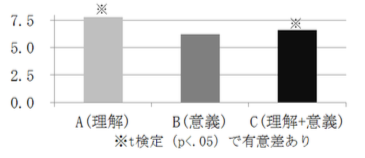
\includegraphics[bb=0 0 365 158, width=7cm]{0710-1.png}
\caption{内発的動機づけの測定結果の差}
\end{figure}

\subsection{内発的動機づけの側面の測定結果の差}

すべてのグループで好奇心と楽しさの側面に有意な向上が見られた.またB,C グループでは帰属の側面も有意に向上した.このことから,学ぶ意義を知るための解説が帰属意識の向上に影響しているといえる.一方で達成,挑戦,因果律の側面は有意に向上しなかった.これは本システムでひとつの学習内容しか扱わなかったことが原因であると考えられる.学習内容のレベルを考慮し,より深い内容や様々な単元を扱うシステムの開発が必要であるといえる.

\begin{figure}[H]
\centering
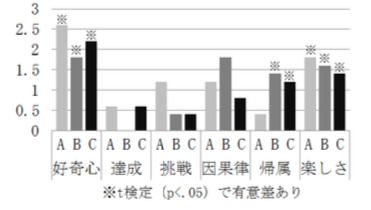
\includegraphics[bb=0 0 370 210, width=7cm]{0710-2.png}
\caption{内発的動機づけの側面の測定結果の差}
\end{figure}

\section{まとめ}
開発したシステムを使用し,理解と学ぶ意義の把握を支援することで学習者の自発的な学習意欲を向上させることができた.
また6つの内発的動機づけの側面のうち好奇心,楽しさの向上には2種類の解説が,帰属の向上には意義を知ることが効果的であることがわかった.



\begin{thebibliography}{99}
\bibitem{system} 門脇直哉,松村敦,宇陀則彦 "自発的な学習意欲を向上させる学習支援システムの開発" , 情報処理学会第75回全国大会, pp.653-654(2013).
\end{thebibliography}

\end{document}